\documentclass[11pt,a4paper]{article}
\usepackage[T1]{fontenc}
\usepackage[utf8]{inputenc}
\usepackage[polish]{babel}
\usepackage{newtxtext,newtxmath}
\usepackage{microtype}
\usepackage[margin=25mm]{geometry}
\usepackage{graphicx}
\usepackage{array,booktabs,tabularx}
\usepackage{amsmath}
\usepackage{titlesec}
\usepackage{caption,float}
\usepackage[unicode,hidelinks]{hyperref}

\hypersetup{
  pdftitle={PONG - przeciwnik uczący się grać. Sprawozdanie},
  pdfauthor={Artur Zamorowski, Kacper Wojtowicz, Rafał Wybraniec},
  pdflang={pl-PL}
}
\graphicspath{{figures/}}
\setlength{\parindent}{0pt}
\setlength{\parskip}{5pt plus 1pt}
\linespread{1.05}
\setlength{\emergencystretch}{1.5em}
\clubpenalty=10000
\widowpenalty=10000
\raggedbottom
\titleformat{\section}{\large\bfseries}{\thesection.}{0.5em}{}
\titleformat{\subsection}{\normalsize\bfseries}{\thesubsection.}{0.5em}{}
\titlespacing*{\section}{0pt}{16pt}{7pt}
\titlespacing*{\subsection}{0pt}{10pt}{4pt}
\captionsetup{font=small,labelfont=normalfont,labelsep=period,justification=centering,skip=6pt,hypcap=false}
\addto\captionspolish{\renewcommand{\figurename}{Rys.}}
\pagestyle{plain}
\newcolumntype{L}[1]{>{\raggedright\arraybackslash}p{#1}}
\newcolumntype{Y}{>{\raggedright\arraybackslash}X}
\newenvironment{reporttable}[1]{%
  \par\smallskip\begingroup\small
  \renewcommand{\arraystretch}{1.2}%
  \setlength{\tabcolsep}{6pt}%
  \tabularx{\linewidth}{#1}\toprule%
}{\bottomrule\endtabularx\endgroup\par\smallskip}

\begin{document}
\begin{center}
{\Large\bfseries PONG: przeciwnik uczący się grać\par}
\vspace{7pt}
Sprawozdanie z projektu nr 1\\
Artur Zamorowski, Kacper Wojtowicz, Rafał Wybraniec\\[5pt]
Sztuczna inteligencja w grach i rozszerzonej rzeczywistości\\
Zespół 1, poniedziałek 8:00--10:15\\
16 listopada 2026 r.
\end{center}

\section{Cel i założenia projektu}

Pong to gra dla dwóch graczy, którzy przesuwają paletki w pionie
po przeciwnych stronach boiska. Każdy z nich próbuje odbić nadlatującą
piłkę i skierować ją poza zasięg przeciwnika. Punkt zdobywa gracz,
którego rywal przepuści piłkę za swoją paletkę.

Celem projektu było przygotowanie przeciwnika, który uczy się sterowania
paletką metodą prób i błędów. Zastosowaliśmy tablicowy Q-learning.
Agent obserwuje sytuację na boisku, wykonuje ruch i otrzymuje nagrodę
za jego skutki. Na tej podstawie aktualizuje zapisaną ocenę swojej decyzji.
Po zakończeniu treningu korzysta z wyuczonej tablicy podczas gry.

Przygotowaliśmy własną symulację 2D, interfejs do gry z człowiekiem
oraz trening uruchamiany bez wyświetlania obrazu. Jako przeciwnika
treningowego i punkt odniesienia przyjęliśmy prostą regułę śledzącą piłkę,
nazwaną w kodzie \texttt{Tracker}. Pracę podzieliliśmy na dwa etapy.
Najpierw przeszukaliśmy 48 kombinacji parametrów agenta ze stanem
siatkowym i wybraliśmy model W32. Jego wyniki stanowią punkt odniesienia.
Następnie zmieniliśmy reprezentację stanu, dodaliśmy rotację piłki
i przeprowadziliśmy dłuższe treningi. Projekt jest zaimplementowany
w Pythonie i obejmuje grę, trening oraz ocenę modeli.
Sprawozdanie przedstawia rozwiązanie bazowe, jego ograniczenia
oraz wyniki uzyskane po usprawnieniach.

\section{Gra i symulacja}

Agent steruje prawą paletką. Lewą paletkę prowadzi człowiek albo
\texttt{Tracker}. Mecz w interfejsie trwa do siedmiu punktów, a każda
wymiana kończy się zdobyciem punktu. Podczas treningu i oceny pojedyncza
wymiana jest osobnym epizodem z limitem 20~s czasu symulowanego.
Przekroczenie tego limitu zapisujemy jako remis.

Na początku epizodu piłka pojawia się na środku szerokości boiska.
Losujemy jej wysokość, kąt i poziomy kierunek lotu oraz początkowe
położenia paletek. Obie paletki mają tę samą maksymalną prędkość
i przyspieszenie. Dzięki temu wynik zależy od sposobu sterowania
przy jednakowych ograniczeniach ruchu.

\begin{figure}[H]
  \centering
  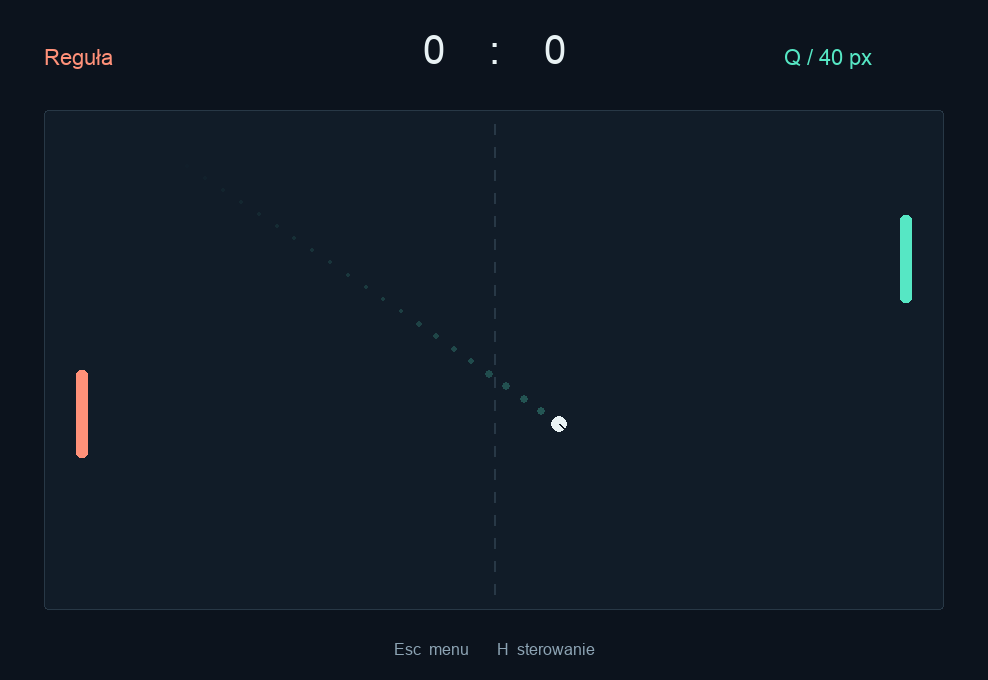
\includegraphics[width=0.72\linewidth]{game.png}
  \caption{Widok gry. W trybie demonstracji lewą paletką steruje \texttt{Tracker}, a prawą wyuczony agent.}
  \label{fig:gra}
\end{figure}

Fizyka działa ze stałym krokiem $1/120$~s. Obaj gracze wybierają ruch
co cztery kroki, czyli 30 razy na sekundę. Paletki stopniowo przyspieszają
i hamują. Piłka odbija się od górnej i dolnej ściany, a po kontakcie
z paletką zwiększa szybkość. Zestaw podstawowych parametrów zawiera
tabela~\ref{tab:fizyka}.

\begin{table}[H]
\caption{Parametry symulacji wspólne dla wszystkich modeli.}
\label{tab:fizyka}
\begin{reporttable}{L{65mm}Y}
\textbf{Parametr} & \textbf{Wartość} \\ \midrule
Rozmiar boiska & $900\times500$~px \\
Rozmiar paletki i promień piłki & $12\times88$~px i 8~px \\
Maksymalna prędkość paletki & 460~px/s \\
Przyspieszenie paletki & 3600~px/s$^2$ \\
Szybkość piłki & Początkowo 430~px/s, maksymalnie 800~px/s \\
Przyspieszenie piłki po odbiciu & Mnożnik szybkości $1{,}06$ \\
\end{reporttable}
\end{table}

Miejsce kontaktu z paletką zmienia kąt odbicia. Trafienie blisko jej
środka daje bardziej poziomy lot, a trafienie bliżej końca zwiększa
pionową składową prędkości. Ruch paletki podczas odbicia wpływa na tę
prędkość i nadaje piłce rotację. Rotacja zakrzywia tor lotu i stopniowo
zanika. Agent musi więc uwzględniać zarówno położenie piłki, jak i jej
ruch oraz bezwładność własnej paletki.

Wykrywanie kolizji uwzględnia ruch piłki między kolejnymi krokami
symulacji. Pozwala to wykrywać odbicia także przy dużej szybkości piłki.

\section{Bazowy agent Q-learning}

\subsection{Obserwacja, stan i akcje}

W modelu bazowym agent wykorzystuje sześć wielkości: pozycję piłki $(x_b,y_b)$,
jej prędkość $(v_x,v_y)$ oraz położenie i prędkość własnej paletki
$(y_p,v_p)$. Te wartości opisują bieżącą sytuację. Agent zamienia je
na dyskretny stan, który wskazuje wiersz tablicy Q.

Pozycje dzielimy przez rozmiar komórki siatki i zaokrąglamy w dół.
Stan zawiera kolumnę i wiersz piłki oraz wiersz paletki. Ruch poziomy
piłki opisujemy znakiem $v_x$. Prędkość pionową piłki dzielimy na trzy
kategorie z progami $-100$ i $100$~px/s, a prędkość paletki na trzy
kategorie z progami $-80$ i $80$~px/s. W efekcie podobne sytuacje
trafiają do tego samego wiersza tablicy.

Porównaliśmy komórki o boku 20, 25, 40 i 50~px. Ich rozmiar określa
liczbę kolumn i wierszy boiska, a przez to liczbę stanów. Dla 50~px
jest to $18\cdot10\cdot10\cdot2\cdot3\cdot3=32\,400$ stanów.
Dla 20~px otrzymujemy $45\cdot25\cdot25\cdot2\cdot3\cdot3=506\,250$.
Dokładniejsza siatka rozróżnia więcej położeń, więc wymaga zebrania
doświadczeń dla większej liczby stanów.

Każdy stan ma trzy możliwe akcje: ruch w górę $a=-1$, postój $a=0$
i ruch w dół $a=1$. Tablica Q ma zatem trzy kolumny. Po zakończeniu
uczenia agent wybiera akcję o największej wartości w bieżącym wierszu.
Gdy postój ma tę samą wartość co najlepszy ruch, wybiera postój.

\subsection{Nagrody i aktualizacja tablicy}

Nagroda wiąże decyzje agenta z wynikiem gry. Przyjęliśmy $+1$ za zdobycie
punktu i $-1$ za jego stratę. Porównaliśmy dwa ustawienia nagrody za
odbicie własną paletką: 0 i $+0{,}2$. W drugim przypadku agent otrzymuje
informację zwrotną także podczas trwania wymiany. W pierwszym musi
powiązać swoje ruchy z nagrodą przyznaną dopiero po rozstrzygnięciu punktu.

Na początku cała tablica Q zawiera zera. Po wykonaniu akcji $a$ w stanie
$s$ agent otrzymuje nagrodę $r$ i obserwuje następny stan $s'$. Wtedy
aktualizuje jedną komórkę zgodnie ze wzorem:
\begin{equation}
Q(s,a)\leftarrow Q(s,a)+\alpha\left[r+\gamma\max_{a'}Q(s',a')-Q(s,a)\right].
\label{eq:qlearning}
\end{equation}
Współczynnik $\alpha$ określa siłę zmiany dotychczasowej oceny, a
$\gamma$ wagę przyszłych nagród. Te współczynniki były parametrami
przeszukiwania. Składnik $\max_{a'}Q(s',a')$ przenosi informację o wartości następnego
stanu do stanu poprzedniego. W kolejnych epizodach agent może więc
nauczyć się ruchu, który dopiero po pewnym czasie umożliwi odbicie.

Po zdobyciu lub stracie punktu epizod kończy się i cel aktualizacji
wynosi samo $r$. Po przerwaniu przez limit czasu zachowujemy składnik
przyszłej wartości, ponieważ gra została zatrzymana w trakcie wymiany.
Aktualizacja odbywa się również wtedy, gdy po ruchu obserwacja nadal
należy do tego samego stanu siatkowego.

\section{Eksperyment bazowy}
\label{sec:baza}

\subsection{Trening i wybór modelu}

Podczas treningu lewą paletką steruje \texttt{Tracker}. Porównuje
wysokość piłki ze środkiem swojej paletki i porusza się w jej stronę;
w zakresie $[-12,12]$~px wybiera postój. Reguła jest stała i podlega
tym samym ograniczeniom ruchu co agent. Doświadczenia powstają
w symulacji: po każdej decyzji agent otrzymuje nagrodę i aktualizuje Q.
W strategii epsilon-greedy z prawdopodobieństwem $\epsilon$ losuje
akcję, a w pozostałych przypadkach wybiera najlepszą. W pierwszym
etapie $\epsilon$ malał liniowo z 0,9 do 0,02 przez 50\,000 epizodów,
potem pozostawał stały.

Przeszukiwanie obejmowało komórki 20, 25, 40 i 50~px,
$\alpha\in\{0{,}03;0{,}12\}$, $\gamma\in\{0{,}98;0{,}995;0{,}999\}$
oraz nagrodę za odbicie 0 lub $+0{,}2$. Dało to 48 kombinacji.
Wszystkie trenowaliśmy do 50\,000 epizodów, osiem
najlepszych do 200\,000, a trzech finalistów do 500\,000.
Każde ustawienie finałowe sprawdziliśmy w trzech niezależnych
treningach. Łącznie wykonaliśmy 7,5 mln epizodów treningowych.

Checkpointy ocenialiśmy na 400 wspólnych serwisach i zachowywaliśmy
najlepszą politykę z każdego
treningu. Przy równym udziale wygranych rozstrzygały mniejszy udział
porażek, a następnie większa liczba odbić. Osobne 2000 serwisów
służyło do wyboru wariantu według średniej z trzech treningów,
a potem jego reprezentanta.
Podczas wszystkich ocen $\epsilon=0$ i tablica Q pozostawała bez zmian.

Po 50\,000 epizodów najlepszy checkpoint osiągnął 15,5\% wygranych;
bez nagrody za odbicie najlepszy wynik wynosił 0,75\%.
Dokładniejsze siatki 20 i 25~px uzyskały najwyżej 0,75\% i 3,5\%.
Dłuższy trening poprawił grę, ale postęp nie był monotoniczny
(rys.~\ref{fig:uczenie}). Uzasadniało to zachowywanie najlepszego
checkpointu zamiast automatycznego wybierania ostatniej tablicy.

\begin{figure}[H]
\centering
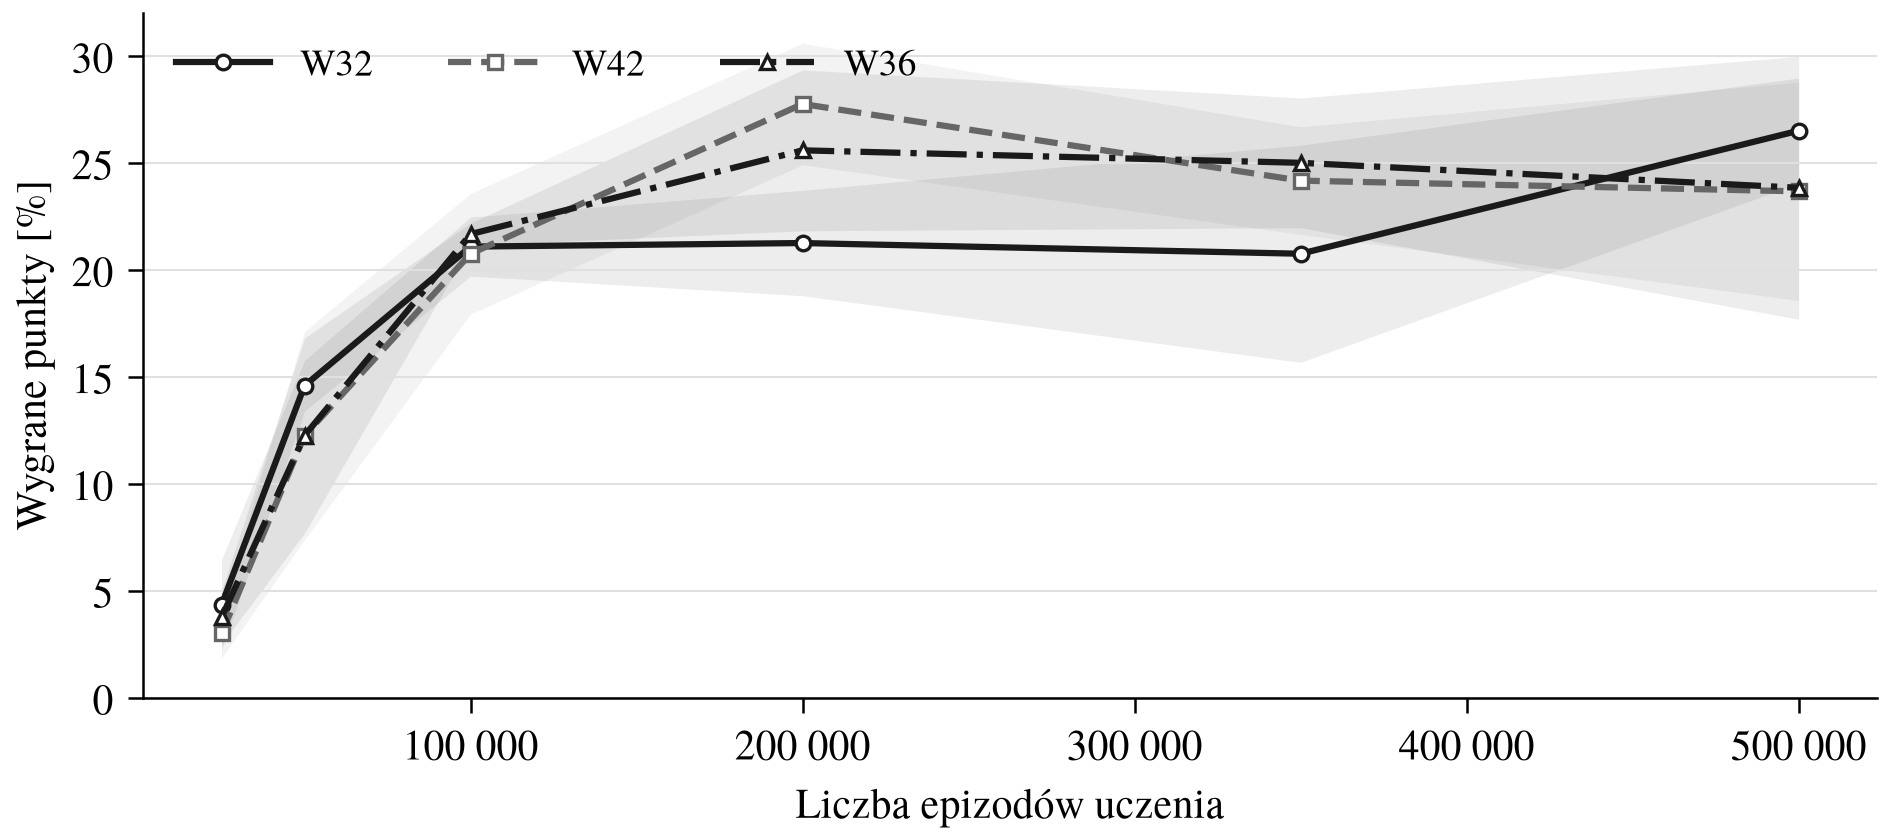
\includegraphics[width=\linewidth]{learning.png}
\caption{Walidacja finalistów eksperymentu bazowego. Linie oznaczają średnie z trzech treningów, a pasma jedno odchylenie standardowe. Każdy pomiar obejmuje 400 epizodów.}
\label{fig:uczenie}
\end{figure}

\subsection{Wyniki modelu bazowego}

W pomiarze wyboru najwyższą średnią uzyskał W32
(tab.~\ref{tab:finalisci}). Jego reprezentantem został checkpoint
po 500\,000 epizodów, który wygrał 28,55\% z 2000 serwisów.

\begin{table}[H]
\caption{Finaliści i średni udział wygranych w pomiarze wyboru na 2000 serwisach. Każdy wariant obejmuje trzy niezależne treningi. Nagroda za odbicie wynosiła $+0{,}2$.}
\label{tab:finalisci}
\begin{reporttable}{Yrrrr}
\textbf{Wariant} & \textbf{Komórka [px]} & $\boldsymbol{\alpha}$ & $\boldsymbol{\gamma}$ & \textbf{Wygrane [\%]} \\ \midrule
W32 & 40 & 0,12 & 0,98 & 26,8 \\
W42 & 50 & 0,03 & 0,999 & 26,0 \\
W36 & 40 & 0,12 & 0,999 & 25,2 \\
\end{reporttable}
\end{table}

Ocena końcowa pierwszego etapu objęła 5000 nowych serwisów na model.
Sprawdziliśmy dziewięć tablic finalistów,
wcześniejszy model z siatką 50~px oraz Trackera sterującego prawą
paletką, zawsze przeciwko lewemu Trackerowi.
Udziały wygranych i strat liczymy względem wszystkich
prób, łącznie z remisami po limicie 20~s. Tabela~\ref{tab:wyniki}
przedstawia wyniki tego etapu; dla finalistów podaje średnie z trzech
treningów i odchylenie standardowe udziału wygranych w punktach procentowych.

\begin{table}[H]
\caption{Ocena końcowa na 5000 serwisach na model. Odbicia oznaczają średnią łączną liczbę odbić obu paletek w epizodzie.}
\label{tab:wyniki}
\begin{reporttable}{Yrrrr}
\textbf{Wariant} & \textbf{Wygrane [\%]} & \textbf{Straty [\%]} & \textbf{Remisy [\%]} & \textbf{Odbicia} \\ \midrule
W32 & $26{,}6\pm2{,}5$ & 50,1 & 23,3 & 9,31 \\
W42 & $26{,}5\pm2{,}9$ & 56,5 & 17,0 & 8,75 \\
W36 & $24{,}4\pm0{,}5$ & 56,3 & 19,3 & 8,76 \\
Wcześniejszy model & 15,2 & 76,1 & 8,7 & 6,71 \\
Tracker & 18,1 & 34,4 & 47,5 & 12,45 \\
\end{reporttable}
\end{table}

Wybrany W32 wygrał 1432 z 5000 prób (28,64\%),
przegrał 2412 (48,24\%), a 1156 zakończył limitem czasu (23,12\%).
Wcześniejszy model wygrał 758 prób (15,16\%) i przegrał 3805.
Poprawa udziału wygranych wyniosła 13,48 punktu procentowego;
średnia liczba odbić wzrosła z 6,71 do 9,35, a czas epizodu
z 12,25 do 15,73~s. W32 i W42 uzyskały zbliżone średnie,
z różnicą mniejszą od rozrzutu między treningami. Tracker miał mniej
porażek i więcej remisów niż W32, więc wyższy udział wygranych
agenta nie oznaczał jeszcze lepszego utrzymywania piłki w grze.

\subsection{Ograniczenia rozwiązania bazowego}

Jedna komórka siatki łączy różne położenia piłki, które mogą wymagać
innych ruchów. Model bazowy opisuje prędkość poziomą tylko znakiem,
a pionową jedną z trzech kategorii. Pomija też rotację, choć wpływa
ona na dalszy tor lotu. Dwie obserwacje zakodowane jako ten sam stan
mogą więc prowadzić do różnych sytuacji przy paletce.

Samo zmniejszenie komórki z 50 do 20~px zwiększa liczbę stanów
około 15,6 razy. Krótkie treningi mogą nie zebrać dla nich wystarczająco
wielu doświadczeń. Pierwszy odsiew na pojedynczym treningu mógł również
odrzucić warianty wymagające dłuższego uczenia. W kolejnym etapie
zmieniliśmy zatem sposób opisu sytuacji i zwiększyliśmy budżet treningu,
zachowując W32 jako punkt odniesienia.

\section{Usprawnienie modelu}
\label{sec:usprawnienia}

\subsection{Stan względny, rotacja i symetria}

Nowy agent nadal korzysta z tablicowego Q-learningu i trzech tych
samych akcji. Obserwuje siedem bieżących wielkości:
$(x_b,y_b,v_x,v_y,y_p,v_p,\omega)$, gdzie $\omega$ oznacza rotację
piłki. Nie otrzymuje przewidywanego miejsca odbicia, czasu do kolizji
ani akcji wyznaczonych przez regułę. Decyzje podczas gry wynikają
z wyuczonej tablicy Q.

W nowym stanie osobny wiersz paletki zastąpiliśmy
różnicą wysokości $y_b-y_p$. Przedziały tej różnicy są gęstsze blisko
zera, a przedziały pozycji poziomej piłki przy prawej paletce.
Dzięki temu tablica dokładniej rozróżnia sytuacje tuż przed odbiciem.
Rozszerzyliśmy też opis prędkości i dodaliśmy pięć kategorii rotacji.
Porównanie z wybranym modelem bazowym zawiera tabela~\ref{tab:stany}.

\begin{table}[H]
\caption{Reprezentacje stanu wybranych modeli. Rozmiary dotyczą W32 oraz nowego modelu z podziałem wysokości co 25~px.}
\label{tab:stany}
\begin{reporttable}{L{40mm}YY}
\textbf{Składnik} & \textbf{Model bazowy W32} & \textbf{Nowy model} \\ \midrule
Pozycja pozioma piłki & Równa siatka 40~px & 8 nierównych przedziałów \\
Pozycje pionowe & Wiersz piłki i wiersz paletki, co 40~px & Wysokość piłki co 25~px i 20 przedziałów $y_b-y_p$ \\
Prędkość pozioma piłki & 2 kategorie kierunku & 4 przedziały \\
Prędkość pionowa piłki & 3 przedziały & 7 przedziałów \\
Prędkość paletki & 3 przedziały & 5 przedziałów \\
Rotacja piłki & Pomijana & 5 przedziałów \\
Symetria góra--dół & Osobne stany & Wspólny wiersz Q, odwrócone akcje \\
Liczba wierszy Q & 69\,966 & 1\,120\,000 \\
\end{reporttable}
\end{table}

Wykorzystaliśmy symetrię fizyki względem poziomej osi boiska.
Dla piłki poniżej środka odbijamy wysokości $y_b$ i $y_p$ względem
wysokości boiska $H$ oraz zmieniamy znaki $v_y$, $v_p$ i $\omega$.
Pozycja $x_b$ i prędkość $v_x$ pozostają takie same. Odbite sytuacje
korzystają z tego samego wiersza Q, a ruch w górę zamienia się
z ruchem w dół. Odwrócenie uwzględniamy zarówno przy wyborze akcji,
jak i aktualizacji tablicy.

Symetria współdzieli doświadczenia, lecz dokładniejszy opis ruchu
i rotacji zwiększa tablicę do 1\,120\,000 wierszy. Większa liczba
rozróżnianych sytuacji wymaga zebrania większej liczby doświadczeń.

\subsection{Eksperyment i wybór modelu}

Sprawdziliśmy sześć konfiguracji: podział wysokości co 25 lub 50~px,
$\alpha=0{,}15$ oraz $\gamma\in\{0{,}98;0{,}995;0{,}999\}$.
Każda otrzymała budżet 2 mln epizodów. Najlepsze ustawienie
sprawdziliśmy w dwóch dodatkowych, niezależnych treningach. Każdy
przebieg zaczynał od zerowej tablicy. Nagrody wynosiły $+1$ za punkt, $-1$
za stratę i $+0{,}2$ za odbicie. Epsilon malał liniowo z 0,7 do 0,02
przez pierwsze 100\,000 epizodów. Przeciwnik, fizyka, częstotliwość
decyzji i limit 20~s pozostały wspólne dla porównywanych modeli.

Co 100\,000 epizodów ocenialiśmy checkpoint na 400 serwisach.
Zachowywaliśmy tablicę o największym
udziale wygranych, przy remisie preferując mniej strat.
Na osobnych 2000 serwisach wybraliśmy konfigurację,
a następnie jej reprezentanta spośród trzech
treningu. W odróżnieniu od eksperymentu bazowego o wyborze konfiguracji
decydował tu wynik pojedynczego przebiegu; dodatkowe dwa treningi
sprawdzały powtarzalność wybranego ustawienia.

Wybrane ustawienie ma podział wysokości co 25~px,
$\alpha=0{,}15$ i $\gamma=0{,}995$. Jego reprezentant uzyskał
49,30\% wygranych w pomiarze wyboru. Wybrana tablica pochodzi
z 1,8 mln epizodów, mimo budżetu 2 mln.
Rysunek~\ref{fig:nowe_uczenie} pokazuje wyniki walidacji w trakcie
uczenia, a nie ocenę końcową wybranych checkpointów.

\begin{figure}[H]
\centering
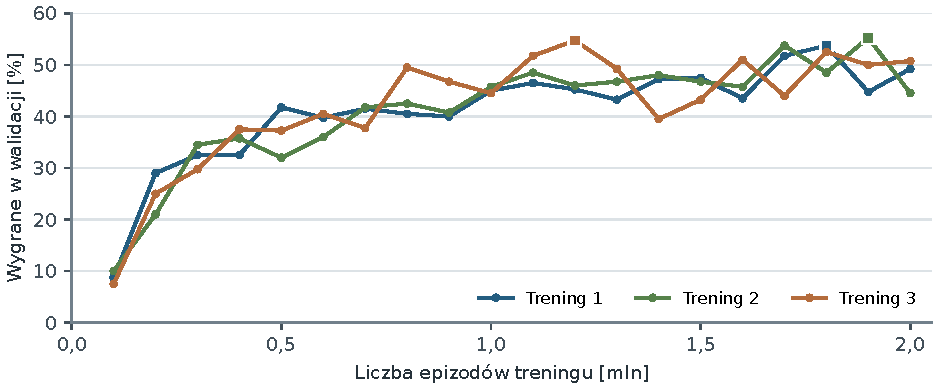
\includegraphics[width=\linewidth]{figures/improved_learning.pdf}
\caption{Walidacja nowego ustawienia w trzech niezależnych treningach. Każdy punkt obejmuje 400 wspólnych serwisów, a kwadraty wskazują checkpointy wybrane do dalszej oceny.}
\label{fig:nowe_uczenie}
\end{figure}

\subsection{Ocena punktowa i porównanie z W32}

Po wyborze modelu oceniliśmy trzy nowe tablice, W32 oraz Trackera
na tych samych 5000 nowych serwisów. Zestaw ten jest rozłączny
z walidacją i pomiarem wyboru. Podczas testu agent korzystał
z wyuczonej polityki bez losowych akcji i dalszego uczenia. Wyniki zawiera
tabela~\ref{tab:nowe_wyniki}.

\begin{table}[H]
\caption{Ocena końcowa na 5000 serwisach na model. Wybrany model i dwa powtórzenia pochodzą z niezależnych treningów tej samej konfiguracji. Odbicia i czas są średnimi na epizod.}
\label{tab:nowe_wyniki}
\begin{reporttable}{Yrrrrr}
\textbf{Model} & \textbf{Wygrane [\%]} & \textbf{Straty [\%]} & \textbf{Remisy [\%]} & \textbf{Odbicia} & \textbf{Czas [s]} \\ \midrule
Wybrany model & 50,24 & 24,56 & 25,20 & 9,65 & 17,39 \\
Powtórzenie 1 & 49,58 & 22,42 & 28,00 & 9,65 & 17,47 \\
Powtórzenie 2 & 48,36 & 29,70 & 21,94 & 9,35 & 17,03 \\
Średnia nowego & 49,39 & 25,56 & 25,05 & 9,55 & 17,29 \\
\midrule
Bazowy W32 & 27,86 & 48,74 & 23,40 & 9,35 & 15,70 \\
Tracker & 17,32 & 35,96 & 46,72 & 12,41 & 18,22 \\
\end{reporttable}
\end{table}

Wybrany nowy model wygrał 2512 prób, przegrał 1228, a 1260 wymian
zakończył limitem czasu. W32 wygrał 1393 i przegrał 2437 prób.
Na wspólnym zestawie udział wygranych wzrósł więc o 22,38 punktu
procentowego, a udział strat spadł o 24,18 punktu procentowego
(rys.~\ref{fig:nowe_porownanie}). Średni czas epizodu wzrósł
z 15,70 do 17,39~s, przy niewielkiej zmianie liczby odbić.

Średni udział wygranych z trzech treningów wyniósł
$49{,}39\pm0{,}95$\%, z odchyleniem standardowym z próby wyrażonym
w punktach procentowych. W każdym treningu uzyskaliśmy model
z większą liczbą wygranych niż strat; wynik 50,24\% dotyczy wybranego reprezentanta.

\begin{figure}[H]
\centering
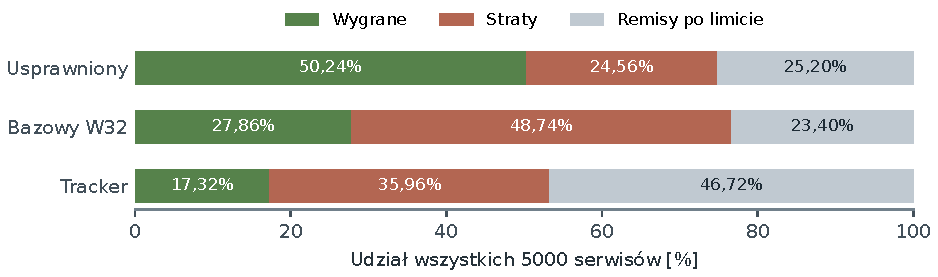
\includegraphics[width=\linewidth]{figures/improved_comparison.pdf}
\caption{Rozkład wyników na wspólnych 5000 serwisach dla usprawnionego modelu, W32 i Trackera. Remis oznacza przekroczenie 20~s, a nie podział punktu w meczu.}
\label{fig:nowe_porownanie}
\end{figure}

W32 uzyskał 28,64\% w eksperymencie bazowym
(rozdział~\ref{sec:baza}) i 27,86\% w porównaniu usprawnień.
Są to pomiary tej samej tablicy na różnych serwisach.
Porównanie modeli opieramy na wspólnym zestawie testowym.

\subsection{Pełne mecze do siedmiu punktów}

Dodatkowo sprawdziliśmy wybrany model w 100 pełnych meczach
przeciwko Trackerowi. Mecz trwał do siedmiu punktów, a każda wymiana
do zdobycia punktu, bez limitu 20~s.

Agent wygrał 89 meczów i przegrał 11, zdobywając łącznie 673 punkty
przy 352 punktach Trackera. Daje to 89\% zwycięstw meczowych.
Ocena punktowa mierzy wynik pojedynczej losowanej wymiany z limitem
czasu, a meczowa zwycięstwo w grze do siedmiu punktów i bez tego
limitu. Dlatego 89\% zwycięstw meczowych i 50,24\% wygranych epizodów
opisują różne warunki gry.

\section{Ograniczenia i wnioski}

W pierwszym etapie dobór parametrów i dłuższy trening zwiększyły
udział wygranych z 15,16\% do 28,64\%. W32 stał się punktem
odniesienia dla dalszych zmian. Nowy opis stanu wraz ze zmianą
parametrów i większym budżetem pozwolił następnie uzyskać 50,24\%
wygranych wobec 27,86\% W32 na wspólnych serwisach. Średnia z trzech
treningów wyniosła 49,39\%, a reprezentant wygrał 89 ze 100 pełnych meczów.

Zmiany ocenialiśmy łącznie, więc nie wyznaczyliśmy osobnego wpływu
rotacji, symetrii i długości treningu.
Stan nadal jest dyskretny i pomija paletkę przeciwnika,
a powtarzalność sprawdzono tylko dla wybranej konfiguracji.
Dalsze prace powinny objąć innych przeciwników i kontrolowane
porównania poszczególnych zmian przy tym samym budżecie treningu.

\section*{Podział prac}

Artur Zamorowski odpowiadał za budowę i trening modelu bazowego.
Kacper Wojtowicz usprawnił model względem wariantu bazowego
oraz przygotował interfejs graficzny i prezentację.
Rafał Wybraniec przygotował silnik gry, opracował sprawozdanie
i dobierał parametry.

\end{document}
